\documentclass[a4paper]{report}

\usepackage[textwidth=14cm]{geometry}
\usepackage{xcolor}
\usepackage{hyperref}
\usepackage{amsmath,amssymb,amsthm}
\usepackage{tikz-cd}
\usepackage{graphicx}

% Theorem environments
\newtheorem{theorem}{Theorem}[section]
\newtheorem{lemma}[theorem]{Lemma}
\newtheorem{proposition}[theorem]{Proposition}
\newtheorem{corollary}[theorem]{Corollary}

\theoremstyle{definition}
\newtheorem{definition}[theorem]{Definition}
\newtheorem{example}[theorem]{Example}

\theoremstyle{remark}
\newtheorem{remark}[theorem]{Remark}

% Lean commands for blueprint tracking
\usepackage{blueprint}

\title{Formalization of Ricci Flow in Lean 4}
\author{RicciFlow Project}
\date{\today}

\begin{document}

\maketitle

\tableofcontents

\chapter{Introduction}

This project aims to formalize the theory of Ricci Flow in Lean 4, building upon the Mathlib library. The Ricci Flow is a powerful tool in differential geometry, introduced by Richard Hamilton and famously used by Grigori Perelman in his proof of the Poincaré conjecture.

The formalization is organized into several modules, each handling different aspects of the theory:
\begin{itemize}
\item Basic definitions and topological foundations
\item Riemannian manifolds and metric tensors
\item Ricci curvature tensors
\item The Ricci Flow equation and existence theorems
\end{itemize}

\chapter{Basic Definitions}
\label{chap:basic}

\begin{definition}[Manifold Type]
\label{def:manifold-type}
\lean{RicciFlow.Basic}
\leanok
We work with a type $M$ equipped with a topological space structure and a charted space structure modeled on $\mathbb{R}$.
\end{definition}

\chapter{Riemannian Manifolds}
\label{chap:riemannian}

\begin{definition}[Riemannian Metric]
\label{def:riemannian-metric}
\lean{RicciFlow.RiemannianMetric}
\uses{def:manifold-type}
A Riemannian metric on a manifold $M$ is a smooth, positive-definite metric tensor field.
\end{definition}

\begin{remark}
The current implementation provides the structure definition. The detailed properties of the metric tensor (smoothness, positive-definiteness) are to be formalized.
\end{remark}

\chapter{Ricci Curvature}
\label{chap:ricci}

\begin{definition}[Ricci Tensor]
\label{def:ricci-tensor}
\lean{RicciFlow.RicciTensor}
\uses{def:riemannian-metric}
The Ricci curvature tensor is obtained by contracting the Riemann curvature tensor.
\end{definition}

\begin{definition}[Scalar Curvature]
\label{def:scalar-curvature}
\lean{RicciFlow.scalarCurvature}
\uses{def:ricci-tensor}
The scalar curvature is the trace of the Ricci tensor with respect to the metric.
\end{definition}

\chapter{Ricci Flow}
\label{chap:flow}

\begin{definition}[Ricci Flow Equation]
\label{def:ricci-flow-equation}
\lean{RicciFlow.ricci_flow_equation}
\uses{def:riemannian-metric, def:ricci-tensor}
The Ricci Flow equation is the geometric evolution equation:
\[
\frac{\partial g}{\partial t} = -2 \operatorname{Ric}(g)
\]
where $g(t)$ is a time-dependent family of Riemannian metrics and $\operatorname{Ric}(g)$ is the Ricci curvature tensor.
\end{definition}

\begin{theorem}[Short-Time Existence]
\label{thm:short-time-existence}
\lean{RicciFlow.short_time_existence}
\uses{def:ricci-flow-equation}
Let $(M, g_0)$ be a compact Riemannian manifold. Then there exists a time $T > 0$ and a smooth family of metrics $g(t)$ for $t \in [0, T)$ such that:
\begin{enumerate}
\item $g(0) = g_0$
\item $g(t)$ satisfies the Ricci Flow equation for all $t \in (0, T)$
\end{enumerate}
\end{theorem}

\begin{proof}
\leanok
This is a deep result in geometric analysis, relying on the theory of parabolic PDEs. The proof involves:
\begin{itemize}
\item Showing that the Ricci Flow equation is a weakly parabolic system
\item Applying short-time existence theory for parabolic systems
\item Establishing appropriate estimates to ensure smoothness
\end{itemize}

In the Lean formalization, this theorem is currently stated as an axiom. A complete formalization would require developing substantial PDE theory.
\end{proof}

\chapter{Future Directions}

\section{Immediate Goals}
\begin{itemize}
\item Complete the definition of Riemannian metrics with smoothness and positive-definiteness conditions
\item Implement the Ricci tensor using Mathlib's connection and curvature theory
\item Prove basic properties of scalar curvature
\end{itemize}

\section{Long-Term Goals}
\begin{itemize}
\item Formalize Hamilton's maximum principle for the Ricci Flow
\item Prove convergence results for special cases (e.g., spheres)
\item Develop the theory of Ricci solitons
\end{itemize}

\appendix

\chapter{Dependency Graph}

The following graph shows the logical dependencies between definitions and theorems in this formalization:

\begin{center}
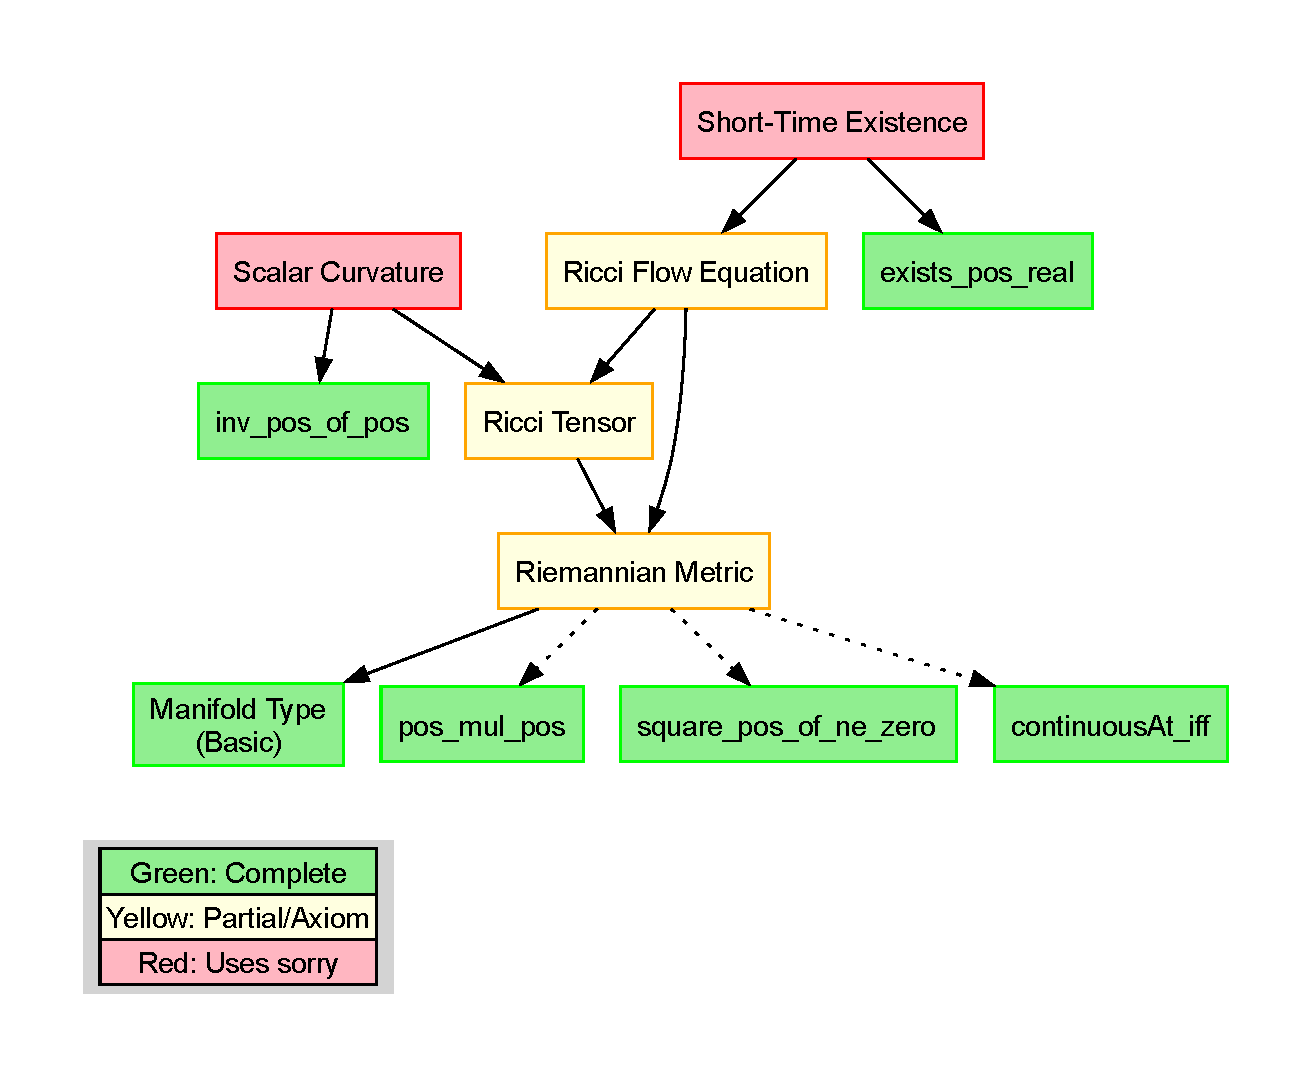
\includegraphics[width=\textwidth]{dep_graph.pdf}
\end{center}

\end{document}
